\chapter{The Cox Proportional Hazards Model \label{chapter:cox}}

We just encountered the Kaplan-Meier estimate of the survival function in Chapter~\ref{chapter:km}. Now we are going to talk about models that treat the Kaplan-Meier curve as the \emph{outcome} in a supervised learning problem. That's right: instead of an outcome that is a number or a category, the survival function itself is the outcome. These models are called \textbf{Cox proportional hazards models}.

\section{Case Study: Ovarian Cancer Survival Data}

We have data from a 1979 study that compares the effect of two different treatments for ovarian cancer\footnote{Edmunson, J.H., Fleming, T.R., Decker, D.G., Malkasian, G.D., Jefferies, J.A., Webb, M.J., and Kvols, L.K., Different Chemotherapeutic Sensitivities and Host Factors Affecting Prognosis in Advanced Ovarian Carcinoma vs. Minimal Residual Disease. Cancer Treatment Reports, 63:241-47, 1979.}. This dataset is in the \texttt{survival} R package under the heading \texttt{ovarian}. 

\section{Dataset}

The dataset contains information on the following variables for $n=26$ women:

\begin{itemize}
\item \emph{futime}: The number of days from enrollment until death or censoring, whichever came first.
\item \emph{fustat}: An indicator of death (1) or censoring (0).
\item \emph{age}: Patient's age in years at time of treatment initiation. 
\item \emph{resid.ds}: An indicator of the extent of residual disease.
\item \emph{rx}: Treatment group (1 = cyclophosphamide, 2 = cyclophosphamide plus adriamycin)
\item \emph{ecog.ps}: A measure of performance score or functional status, using the Eastern Cooperative Oncology Group (ECOG)'s scale. It ranges from 0 (fully functional) to 4 (completely disabled). Level 4 subjects are generally considered to be too ill to enter a randomized trial such as this.
\end{itemize}

\begin{center}
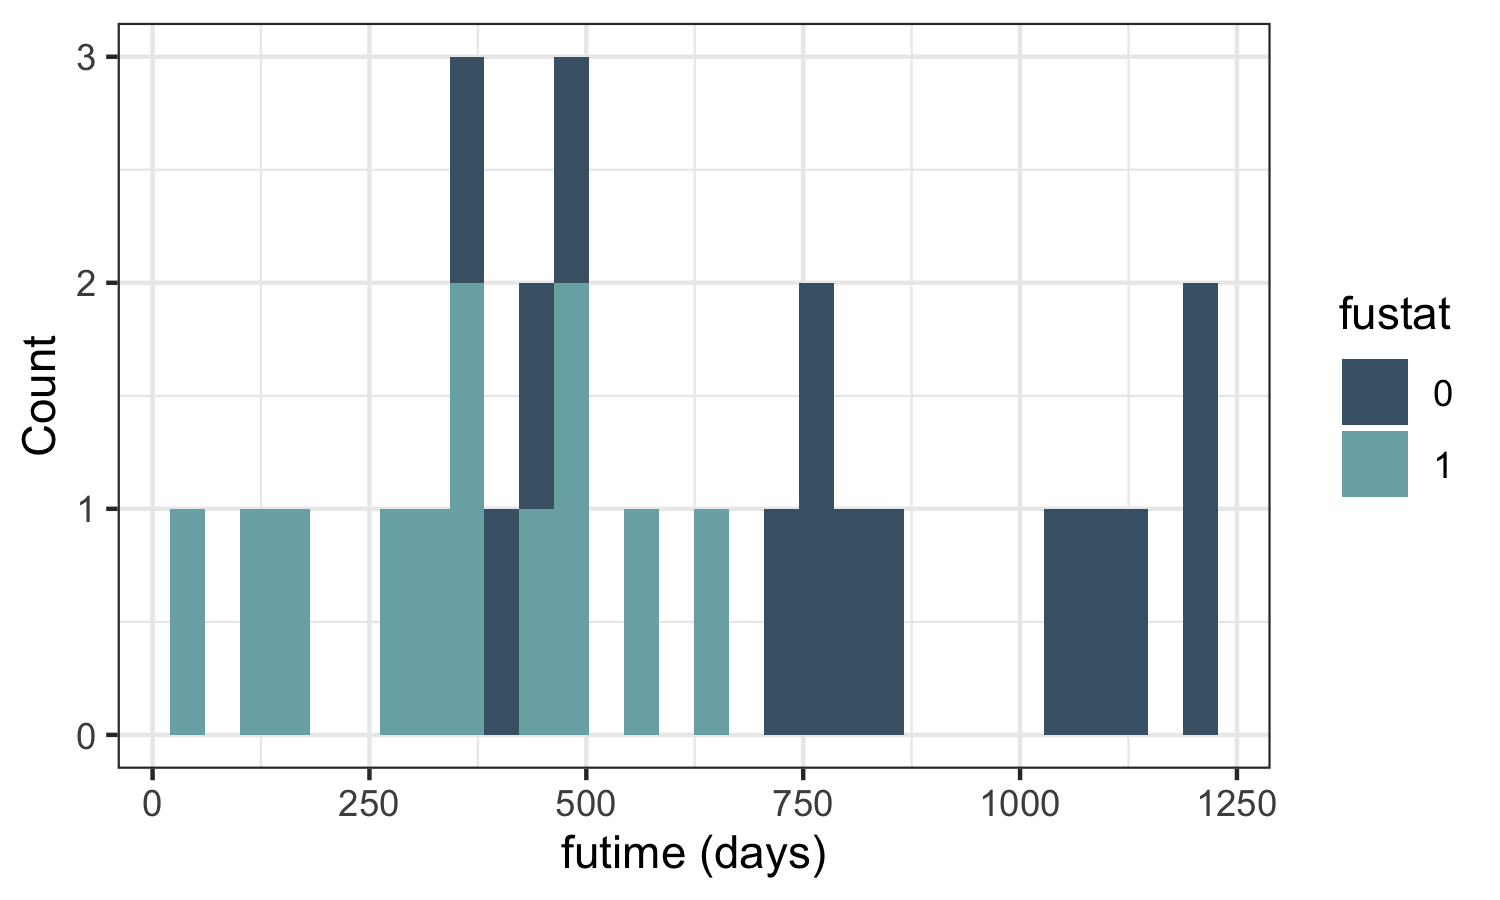
\includegraphics[width=0.3\textwidth]{img/cs-ovarian-futime.png}
\end{center}

\section{Questions}

\section{Analysis}





\subsection{Consideration \#1: What to do with Missing Subjects?}

Imagine creating a logistic regression model for which the outcome is death vs. no death by a particular timepoint. What should you do with patients who left the study before that time? The most na\"ive approach might assign them an outcome of 0 (no death). 

This is not a great strategy because we don't actually know what happened to these people once they left the study. We are effectively making up data for them, and this problem becomes more acute as our timepoint for evaluation becomes longer. At $1000$ days post-treatment, for example, there are only four patients remaining. We would be making up an outcome of ``no death'' for the $9$~patients who left the study before that time -- essentially inventing information for $9/26 = 34.6$\% of our patients. This is unlikely to lead to an accurate estimate of treatment effect.

While this approach is almost never seen in traditional clinical studies, it is used all the time when machine learning models are applied to EHR data. For example, most studies that use machine learning models to predict binary outcomes (e.g., death vs. no death within 30 days) from EHR data treat patients who have left the health system as negative training examples.

\subsection{Consideration \#2: Is a Yes/No Outcome Really Appropriate?}

Okay, so what if we simply don't include patients who leave the study? We could choose to analyze only those patients who are still in the study or who have experienced the outcome (in this case, death) prior to the evaluation time. This avoids the problem of making up data for censored patients, but it also has the effect of changing the number and composition of subjects in the study. Our interpretation of the data is at risk of bias unless the censoring process is completely random\footnote{See the definition of ``missing completely at random (MCAR)'' in Chapter~\ref{chapter:missingdata}. Ignoring censored observations is akin to performing an analysis using only complete data.} and unrelated to the outcome or predictors under study.

In addition, this approach requires us to choose an evaluation time. Here are the results of nine different logistic regression models with different evaluation times on the \texttt{ovarian} dataset:
\begin{center}
{\small
\begin{tabular}{cccc}
  \toprule
  Evaluation Time (days) & Coefficient on \texttt{rx=2} & $p$-Value & Number of Subjects \\ 
  \midrule
  200 & -19.3621 & 0.9969 & 26 \\ 
  300 & -18.7551 & 0.9950 & 26 \\ 
  400 & -1.1394 & 0.2361 & 25 \\ 
  500 & -0.7419 & 0.3946 & 22 \\ 
  600 & -0.3646 & 0.6702 & 22 \\ 
  700 & -0.7419 & 0.3946 & 22 \\ 
  800 & -0.0488 & 0.9596 & 19 \\ 
  900 & -0.7419 & 0.4939 & 17 \\ 
  1000 & -0.7419 & 0.4939 & 17 \\ 
  \bottomrule
\end{tabular}
}
\end{center}
Depending on the specifics of our dataset, our model interpretation could change dramatically depending on which time we choose for the evaluation. In the \texttt{ovarian} dataset, several members of the \texttt{rx=1} group pass away early. This makes treatment $2$ look highly protective at shorter evaluation times, whereas its effect fades at longer evaluation times.

The more important question, however, is whether a yes/no death/no-death outcome actually captures what we want to know about this dataset. Using logistic regression here throws away a tremendous amount of information because a patient who dies early and one who dies the day before the evaluation time are treated exactly the same. 

What we really want to know is whether treatment $2$ \emph{prolongs survival} of ovarian cancer patients relative to treatment $1$. We would like a way to summarize the overall effect of the treatment group on survival time without having to perform separate analyses at multiple different timepoints. This is where survival analysis comes in.